\documentclass{article}
\usepackage{amsmath}


%encoding
%--------------------------------------

%----------------------------
\usepackage{microtype}
%\usepackage{fourier}
\usepackage{helvet}
\usepackage{arevtext,arevmath}

\usepackage[utf8]{inputenc}
\usepackage[T1]{fontenc}

\usepackage{mathastext}
%units
%--------------------------------------
\usepackage{siunitx}
%drawing
%------------------------------------
\usepackage{tikz} % To generate the plot from csv
\usepackage{pgfplots}
\usepackage{pgfplotstable}
\usepackage{graphicx}

\usepackage{caption}
\usepackage{color, colortbl}
\usepackage{tabularx}
\usepackage{setspace}
\usepackage{mhchem}
\usepackage{fancyhdr}
\usepackage[landscape]{geometry}
\usepackage{listings}

\pagestyle{fancy}

\cfoot{\thepage}

\rhead{Gruppe 24}
\lhead{\textbf{HPLC - Bestimmung von Coffein in Kaffe} Messergebnisse und Kalibrierreihe}
\setlength{\headheight}{15pt}


\renewcommand{\familydefault}{\sfdefault}

\sisetup{
  round-mode          = places,
  round-precision     = 2,
  inter-unit-product =\ensuremath{{}\cdot{}}
}

\definecolor{LightCyan}{rgb}{0.88,1,1}
\usetikzlibrary{datavisualization}
\pgfplotsset{compat=newest} % Allows to place the legend below plot
\usepgfplotslibrary{units} % Allows to enter the units nicely
\usepackage{overcite}
\renewcommand\citeform[1]{[#1]}

\makeatletter
\setlength{\@fptop}{0pt}
\makeatother
%\usetikzlibrary{arrows, positioning, calc, datavisualization}

\begin{document}
%\begin{luacode*}
function string:split(sep)
        local sep, fields = sep or "%s", {}
        local pattern = string.format("([^%s]+)", sep)
        self:gsub(pattern, function(c) fields[#fields+1] = c end)
        return fields
end

function printHyperbola()
    local lines={}

    for line in io.lines("dampf.csv") do
            table.insert(lines, line)
    end
    tex.sprint("\\addplot[color=black] coordinates{")

    for i=2,#lines do
        local a=lines[i]:split()
        tex.sprint("("..a[1]..","..a[2]..")")
    end
     tex.sprint("};")
    tex.sprint("\\addplot[color=blue] coordinates{")

    for i=2,#lines do
        local a=lines[i]:split()
        tex.sprint("("..a[1]..","..a[3]..")")
    end
     tex.sprint("};")

end
\end{luacode*}
%\begin{figure}
\centering
     \begin{tikzpicture}
            \begin{axis}[standard,xlabel=Temperatur,ylabel=Druck]
                \directlua{printHyperbola()}
            \end{axis}
        \end{tikzpicture}
     \end{figure}

\noindent
\pagenumbering{gobble}

\begin{figure}[!t]



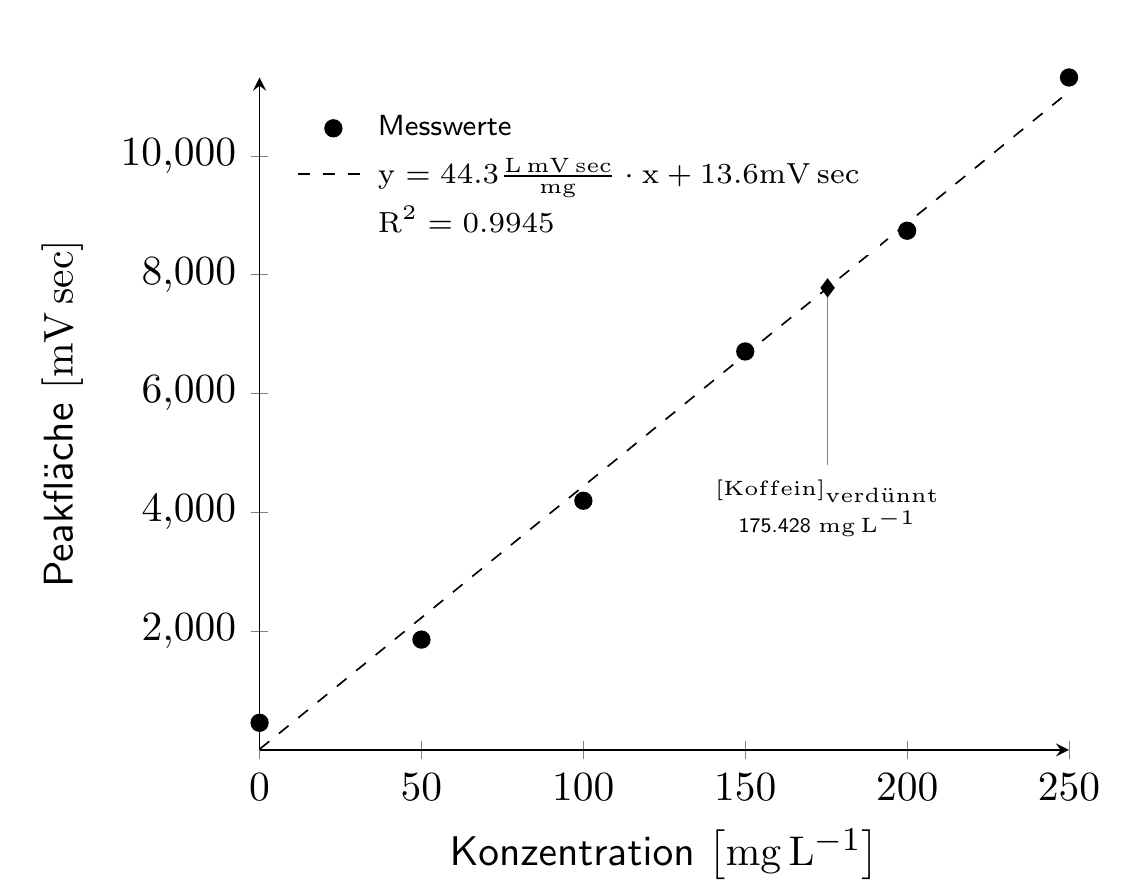
\begin{tikzpicture}[scale=1.5,transform shape]
\begin{axis}[
axis x line=bottom,
axis y line=middle,
xlabel= Konzentration,
ylabel= Peakfläche,
x unit= \si{\milli\gram\per\liter} ,
y unit= \si{\milli\volt.\sec},
legend style={draw=none,legend pos=outer north east},
y label style={at={(axis description cs:-0.2,.5)},rotate=90,anchor=south},
  legend style={legend pos=north west,font=\scriptsize},
  legend cell align=left,
 scaled ticks=false,
  tick label style={/pgf/number format/fixed}
]
\addplot[only marks] table {
  X Y
 0 458.537
 50 1859.115
 100 4196.752
 150 6710.205
 200 8742.891
 250 11323.003
  };
  \node[coordinate,pin={[pin distance=1.5cm]-90:{\tiny $[Koffein]_{verd\ddot{u}nnt}$ }}] at (axis cs:175.428,7781.223) {};
\node[below] at (axis cs:175.428,4281.223) {\tiny 175.428 \si{\milli\gram\per\liter}};
  \addlegendentry{Messwerte }
  \addplot[dashed,domain=0:250] { 44.278*x + 13.624};
\addlegendentry{$y = 44.3  \frac{\si{\liter.\milli\volt.\sec}}{\si{\milli\gram}} \cdot x + 13.6 \si{\milli\volt.\sec}$}
\addplot[draw=none,white] coordinates {(1,1)};
\addlegendentry{ $R^2=0.9945$}
\addplot[only marks,mark=diamond*] coordinates {(175.428,7781.223)};

\end{axis}
\end{tikzpicture}
\caption{Peakflächen in Abhängigkeit der Konzentrationen von Standard-Lösungen}
\end{figure}
\begin{flushleft}
  Das R-Code zur Erstellung der Regressionslinie:
\end{flushleft}
\begin{lstlisting}
assign("c", c(0, 50, 100, 150, 200, 250 ))
assign("p", c(458.537, 1859.115, 4196.752, 6710.205, 8742.891, 11323.003))
fitpc<-lm(p ~ c )
summary(fitpc)
\end{lstlisting}
\end{document}


%\addplot[domain=0:1200]{-1.42e-5*x^(2)+2.836e-2*x+45.47};


